%
% Knihovna pro efektivní nahrávání obrázků na webový server 
% 
% Licensed under MIT License
%

\documentclass[
    monochrome,   % Enables colorful typesetting. Replace with
             % `monochrome`, if you are going to print the
             % thesis on a monochromatic printer.
		table,   % Causes the coloring of tables. Replace with
             % `notable` to restore plain tables.
    twoside, % Enables double-sided typesetting. Replace
             % with `oneside`, if you are going to print
             % your thesis on only one side of the paper.
    % More options are listed in the class documentation
    % available at <https://www.ctan.org/pkg/fithesis>.
]{fithesis/fithesis3}
\usepackage[slovak]{babel} % By using `czech` or `slovak`
% instead of `english`, you can typeset the entire thesis
% in either Czech or Slovak, respectively. Changing the
% language requires a clean compilation; click `recompile
% from scratch`, when Overleaf raises an error.
\thesissetup{
	university    = mu,
	faculty       = fi,
    type          = bc,
    author        = Tomáš Bončo,
    gender        = m,
    advisor       = RNDr. Tomáš Obšívač,
    title         = {Knižnica pre efektívne nahrávanie obrázkov na webový server},
    TeXtitle      = {Knižnica pre efektívne nahrávanie obrázkov na webový server},
    keywords      = {keyword1, keyword2, ...},
    TeXkeywords   = {keyword1, keyword2, \ldots},
}
\thesislong{abstract}{
	This is the abstract of my thesis, which can
    
    span multiple paragraphs.
}
\thesislong{thanks}{
	This is the acknowledgement for my thesis, which can
    span multiple paragraphs.
}

% Page creation engine
\documentclass[11pt,a4paper]{report}
\usepackage[utf8]{inputenc}
\usepackage[slovak]{babel}
\usepackage[T1]{fontenc}


% Main modules
\usepackage{url}      % URL
\usepackage{hyperref} % Links
\usepackage{graphicx} % Pictures
\usepackage{wrapfig}  % In-line Pictures
\usepackage{verbatim} % Code
\usepackage{moreverb} % Encoding
\usepackage{listings} % Code
\usepackage{color}    % Highlight
\usepackage{tikz}
\usepackage[section]{placeins}
\usetikzlibrary{calc,trees,positioning,arrows,chains,shapes.geometric,%
    decorations.pathreplacing,decorations.pathmorphing,shapes,%
    matrix,shapes.symbols}

\usepackage{amsmath}
\usepackage{tabularx}
\usepackage{booktabs}

% Styles
\tikzset{
>=stealth',
  punktchain/.style={
    rectangle, 
    rounded corners, 
    % fill=black!10,
    draw=black, very thick,
    text width=10em, 
    minimum height=3em, 
    text centered, 
    on chain},
  line/.style={draw, thick, <-},
  element/.style={
    tape,
    top color=white,
    bottom color=blue!50!black!60!,
    minimum width=8em,
    draw=blue!40!black!90, very thick,
    text width=10em, 
    minimum height=3.5em, 
    text centered, 
    on chain},
  every join/.style={->, thick,shorten >=1pt},
  decoration={brace},
  tuborg/.style={decorate},
  tubnode/.style={midway, right=2pt},
}


\lstdefinelanguage{JavaScript}{
  keywords={break, case, catch, continue, debugger, default, delete, do, else, false, finally, for, function, if, in, instanceof, new, null, return, switch, this, throw, true, try, typeof, var, void, while, with},
  morecomment=[l]{//},
  morecomment=[s]{/*}{*/},
  morestring=[b]',
  morestring=[b]",
  ndkeywords={class, export, boolean, throw, implements, import, this},
  keywordstyle=\bfseries,
  ndkeywordstyle=\bfseries,
  identifierstyle=\color{black},
  commentstyle=\ttfamily,
  stringstyle=\ttfamily,
  sensitive=true
}

\lstset{ 
  extendedchars=true,
  belowcaptionskip=1\baselineskip,
  breaklines=true,
  xleftmargin=\parindent,
  showstringspaces=false,
  basicstyle=\footnotesize\ttfamily,
  keywordstyle=\bfseries,
  commentstyle=\itshape,
  frame=tb,
  xleftmargin=\fboxsep,
  xrightmargin=-\fboxsep,
  captionpos=b,
 showtabs=false,
}



% Document
\begin{document}

% Chapter files listing
\chapter{Súčasné metódy nahrávania obrázkov}

Aby sa dali veci robiť lepšie a~efektívnejšie, je najprv potrebné preskúmať už vytvorené spôsoby a~uvedomiť si ich nedostatky. Zamedzí sa tak opakovaniu chýb.
  

\section{HTML tag <input\textgreater}

Historicky prvým spôsobom je nepárový tag \emph{<input type="file"\textgreater}. Objavil sa už v~roku 1997, keď konzorcium W3C vydalo štandard \emph{HTML~3.2} \cite{html32}. Umožňuje nahrávanie súborov, a~teda aj obrázkov, ako súčasť zaslaného formulára (musí sa vyskytovať uprostred tagu <form\textgreater). Scenár nahrávania prebieha nasledovne:

\begin{figure}[!hbt]
	\centering
	\begin{tikzpicture}[node distance=.8cm, start chain=going right,]
		\node[punktchain, join] (input) {\emph{<input>} element};
		\node[punktchain, join] (modal) {Zvolenie obrázka z~modálneho okna};
		\node[punktchain, join, on chain=going below] (form-sending) {Odoslanie formulára};
		\node[punktchain, join, on chain=going left] (server-processing) {Spracovanie na~serveri};
	\end{tikzpicture}
	
	\caption{Schéma nahrávania obrázka pomocou \emph{<input>} elementu.}
\end{figure}

\begin{enumerate}
	\item Užívateľ myšou klikne na~\emph{<input>} element.
	\item Vyskočí modálne okno, z~ktorého užívateľ vyberie obrázok.
	\item Užívateľ odošle formulár, obrázok je odoslaný na~server, kde je spracovaný.
\end{enumerate}

Výhody tohto riešenia sú predovšetkým:
\begin{itemize}
	\item Natívna podpora v~prehliadačoch -- nie sú potrebné žiadne ďalšie JavaScriptové súbory.
	\item Jednoduché na~implementáciu.
	\item Podpora \emph{Drag\&Drop}.
\end{itemize}


\section{FormData a~XMLHttpRequest}

\emph{XMLHttpRequest Level 2} pridáva nové rozhranie \emph{FormData}, ktoré umožňuje vytvoriť reprezentáciu formulára v~tvare kľúč-hodnota, čím umožňuje zaslať formulár pomocou \emph{XMLHttpRequest} \cite{MDN_Formdata}. \emph{XMLHttpRequest} je API, ktoré umožňuje prenášať dáta medzi~prehliadačom a~serverom bez~toho, aby nastalo obnovenie stránky \cite{MDN_XMLHttpRequest}.

Vďaka \emph{FormData} je možné odstrániť obmedzenie, kde \emph{<input type="file"\textgreater} musí byť vložený do~formulára (<form\textgreater). Použitím \emph{XMLHttpRequest} eventu \emph{onprogress} je možné sledovať proces nahrávania \cite{MDN_XMLHttpRequest_progress}. Scenár nahrávania môže vyzerať nasledovne:
\begin{enumerate}
	\item Užívateľ myšou klikne na~\emph{<input>} element.
	\item Vyskočí modálne okno, z~ktorého užívateľ vyberie obrázok.
	\item Obrázok sa odošle na~server, zatiaľ čo užívateľ sleduje proces nahrávania. Keď je obrázok plne nahraný a~spracovaný, odošle sa jeho odkaz naspäť užívateľovi do~prehliadača.
	\item Užívateľovi sa zobrazí nahraný obrázok. Pokiaľ s~ním nie je spokojný, postupuje od~bodu 1. Ak je spokojný, odošle formulár. V~tomto prípade nedochádza k~žiadnej manipulácii s~obrázkom.
\end{enumerate}

Výhody tohto riešenia sú predovšetkým:
\begin{itemize}
	\item Nie je potrebné umiestnenie vo formulári.
	\item Je možné zaslať obrázok na~pozadí, čo umožňuje využitie v~moderných webových aplikáciách, kde je obnovenie stránky nežiaduce.
	\item Počas nahrávania je možné zobraziť proces v~percentách.
	\item Po~nahratí obrázka na~server je možné obrázok užívateľovi zobraziť. Takto ho užívateľ vidí pred~potvrdením formulára.
	\item Podpora \emph{Drag\&Drop}.
\end{itemize}

\begin{figure}[!ht]
	\centering
	\begin{tikzpicture}[node distance=.8cm, start chain=going below,]
		\node[punktchain, join] (input) {\emph{<input>} element};
		\node[punktchain, join] (modal) {Modálne okno};
		\node[punktchain, join] (file-choose) {Zvolenie obrázka};
		\node[punktchain, join] (send-file) {Odoslanie obrázka na~server};
		\node[punktchain, join, dashed, on chain=going right] (server-processing) {Spracovanie na~serveri};
		\node[punktchain, join, on chain=going below left] (image-display) {Zobrazenie obrázka};
	\end{tikzpicture}
	
	\caption{Schéma nahrávania obrázka pomocou \emph{<input>} elementu v~kombinácii s~\emph{FormData} a~{XMLHttpRequest}.}
\end{figure}


\section{Riešenia založené na~Adobe Flash a~Microsoft Silverlight}

V dobe písania tejto práce boli stále veľmi rozšírené riešenia, založené na~technológii Adobe Flash (ďalej spomínaný už len ako Flash). Flash, pôvodne navrhnutý pre~tvorbu multimediálneho obsahu -- vektorovej grafiky, animácií, hier pre~prehliadač -- sa stal populárnym aj na~tvorbu väčších aplikácií v~prehliadači, pracovanie so~vstupom z~webovej kamery či mikrofónu, až po~prehrávanie videí a~zvuku.

O~niečo podobné sa pokúšal Microsoft s~technológiou Silverlight (ďalej len Silverlight). Obe technológie nepoužívajú JavaScript, ale iné jazyky -- v~prípade technológie Flash ide o~ActionScript a~v prípade Silverlight ide o~Visual Basic, C\#, Ruby alebo Python. \textbf{V~týchto technológiách by preto bolo možné napísať aj celú našu knižnicu}, avšak nemohli by sme dosiahnuť podporu mobilných zariadení a~obe technológie vyžadujú inštaláciu rozšírení tretích strán do~prehliadača.

Hlavným dôvodom neúspechu technológie Flash a~Silverlight sa stalo odmietnutie podpory od~firmy Apple (pozri \ref{sec:mobile-support}). V~súčasnej dobe nie je podporovaný na~mobilných zariadeniach s~operačným systémom iOS, Android a~Windows Phone. Samotné Adobe už prestáva ďalej Flash podporovať a~zameriava sa radšej na~HTML5 \cite{Flash_dead}.
\graphicspath{ {img/23/} }

\chapter{Nevýhody súčasných metód}
\section{Podpora mobilných zariadení}

V roku 2010, Steve Jobs, spoluzakladateľ a~v tom čase aj výkonný riaditeľ Applu vydal vyhlásenie \emph{Thoughts on Flash}\cite{Apple_flash}, v~ktorom vysvetľuje prečo zariadenia iPhone, iPod a~iPad nepodporujú \emph{Adobe Flash}. Kritizuje \emph{Adobe Flash} z~uzavrenosti, vysokej systémovej záťaže, slabej bezpečnosti a~chýbajúcej podpore dotykových zariadení.
BBC v~roku 2012 informovala\cite{Android_flash}, že Adobe sťahuje \emph{Adobe Flash Player} z~\emph{Google Play store}, čo dovtedy umožňovalo prehrávať \emph{Adobe Flash} na~mobilných zariadeniach. To znamená, že mobilné operačné systémy, ktoré dohromady zaberajú 96,7\% trhu\cite{Mobile_OS_share} nepodporujú \emph{Adobe Flash}.


>> Zdroj hovorí len o~Smartphonoch, nie sú zahrnuté tablety. Použiť radšej: https://www.netmarketshare.com/operating-system-market-share.aspx?qprid=8&qpcustomd=1
>> Nenašiel som žiaden dobrý zdroj, ktorý by priamo vravel, že Silverlight nie je podporovaný na~iOS alebo Androide. Wikipedia rovno hovorí, že Silverlight je zastaraný. Opäť som ale nenašiel žiadne oficiálne tvrdenie.


\section{Zbytočné súbory na~serveri}

Nahrávanie obrázkov bez~toho, aby užívateľ najskôr obrázok videl, môže viesť k~tomu, že užívateľ nahraje nesprávny obrázok. Tak isto môže vzniknúť problém, kde užívateľ kvôli nesprávnemu spracovaniu obrázku na~serveri (napríklad nesprávny orez, pozri \ref{sec:orezanie-obrazka}), môže zmeniť svoje rozhodnutie. Takto vznikajú na~serveri súbory - obrázky, ktoré sa nikdy nepoužijú. Jedno z~riešení tohto problému je pravidelné mazanie nevyužívaných obrázkov.   

\section{Orezanie obrázka}
\label{sec:orezanie-obrazka}

Pri spracovaní na~serveri zvyčajne dochádza k~zmenšeniu a~orezaniu obrázka. Spravidla sa obrázky orezávajú na~stred. To však môže byť nesprávne, ako ukazuje obrázok XX (TODO), kde orezanie na~stred odreže osobu - najdôležitejšiu časť obrázka. Čiastočným riešením je využitie detekcie tvárí. Pokročilé riešenia si však vyžadujú pokročilú analýzu obrazu, kde sa analyzuje kontrast a~hrany. Vďaka tomu je možné detekovať východ slnka, alebo budovu na~obrázku. 

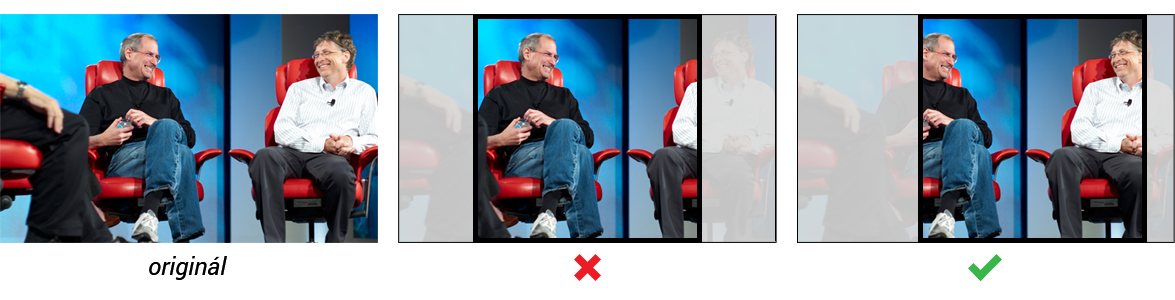
\includegraphics[width=\textwidth]{jobs_gates}

\section{Prenášanie zbytočných dát}

// TODO
\chapter{Vytvorenie knižnice na~nahrávanie obrázkov}
\label{sec:solution}

\section{Ciele}
\label{sec:goals}

Ciele, ktoré sme stanovili pri~vytváraní knižnice majú za~úlohu maximalizovať pohodlie užívateľa, minimalizovať zaťaženie pre~tvorcov stránky a~mala by byť prístupná pre~čo najširšie publikum. Preto sme stanovili, že knižnica by mala:

\begin{itemize}
	\item byť nezávislá od~knižníc/frameworkov tretích strán, napr. \emph{jQuery},
	\item podporovať nahrávanie, či už zvolením obrázka cez~modálne okno alebo aj technológiou \emph{Drag\&Drop}, 
	\item byť jednoduchá na~implementovanie,
	\item byť dobre rozšíriteľná o~nové funkcie,
	\item podporovať nahrávanie bez~obnovenia stránky,
	\item podporovať mobilné zariadenia,
	\item podporovať nahrávanie viacerých obrázkov,
	\item byť dobre zdokumentovaná.
\end{itemize}


\section{Riešenie}
\subsection{Predstavenie}
\label{sec:predstavenie-riesenia}
Najskôr sme plánovali využiť \emph{jQuery}, ale kvôli splneniu prvého cieľa (byť nezávislí od~knižníc/frameworkov tretích strán) sme sa rozhodli využiť \emph{Custom Element}. Vytvorili sme jeden, ktorý slúži na~úpravu obrázka \emph{<x-cupe>} a~jeden na~podporu nahrávania viacerých obrázkov - \emph{<x-cupe-gallery>}. Oba vychádzajú z~rovnakého HTML, pričom \emph{<x-cupe-gallery>} interne využíva \emph{<x-cupe>}, preto sa ďalej v~tejto kapitole zameriame na~element \emph{<x-cupe>}. Nahrávanie viacerých obrázkov je bližšie popísané v~kapitole 3.5.


Scenár nahrávania môže vyzerať takto:
\begin{enumerate}
	\item Užívateľ buď pomocou \emph{Drag\&Drop} nahraje obrázok, alebo klikne na~element a~následne si z~modálneho okna zvolí obrázok.
	\item Obrázok sa zmenší, oreže a~zobrazí.
	\item Pokiaľ užívateľ nie je spokojný s~obrázokom, pokračuje prvým bodom.
	\item Pokiaľ užívateľ nie je spokojný s~orezaním, držaním stlačeného ľavého tlačidla myši posúva obrázok, dokým nie je spokojný.
	\item Keď je užívateľ spokojný s~obrázkom aj jeho orezaním, odošle formulár. Až vtedy sa zmenšená a~orezaná verzia nahraje na~server.
\end{enumerate}

Hoc sa v~scenári spomína klikanie, knižnica podporuje aj dotykové zariadenia, a~teda všetky úkony je možné vykonať dotykom. Interne oba elementy využívajú nasledujúce HTML:

\begin{lstlisting}[language=HTML,caption=Interná štruktúra elementov \emph{<x-cupe>} a~\emph{<x-cupe-gallery>}.]
<canvas></canvas>
<input type="file" style="display: none">
<input type="text" style="display: none">
\end{lstlisting}

% TODO: Fix Listening

Element \emph{<canvas>} sa stará o~zobrazenie obrázka. Na~prácu s~ním sme vytvorili pomocnú triedu \emph{XCupeCanvasElement}, pomocou ktorej vieme rýchlo zmeniť rozmery. Keď užívateľ klikne na~\emph{<x-cupe>}, element deleguje klik na~\emph{<input type="file"\textgreater}, čo spôsobí, že sa otvorí modálne okno a~užívateľ si môže zvoliť obrázok. Pre~zjednodušenie práce s~ním sme vytvorili triedu \emph{XCupeInputFileElement}. Do~\emph{<input type="text"\textgreater} sa vloží textová reprezentácia obrázka, čo umožňuje jeho odoslanie cez~POST. Opäť, aj pre~tento element sme vytvorili pomocnú triedu \emph{XCupeInputFileElement}. Detailné fungovanie knižnice je popísané v~sekcii \ref{sec:upload-and-settings}.

\subsection{Použitie}

Použitie \emph{Custom Elementu} nám umožnuje skutočne jednoduchý spôsob inštalácie, kde sa najskôr načítajú zdrojové súbory knižnice:
\begin{lstlisting}
<link rel="import" href="dist/x-cupe.html">
\end{lstlisting}

Následne stačí už len na~príslušnom mieste v~kóde vytvoriť element:
\begin{lstlisting}
<x-cupe></x-cupe>
\end{lstlisting}

V prípade nahrávania viacerých obrázkov:
\begin{lstlisting}
<x-cupe-gallery></x-cupe-gallery>
\end{lstlisting}

\begin{figure}[!hb]
	\centering
	\begin{tikzpicture}[node distance=.8cm, start chain=going below,]
		\node[punktchain] (file-read) {Prečítanie súboru};
		
			\begin{scope}[start branch=clicking,
			every join/.style={->, thick, shorten <=1pt}, ]
				\node[punktchain, on chain=going above left, join=by {<-}, xshift=2cm]
					(modal) {Výber obrázka z~modálneho okna};
					
				\node[punktchain, on chain=going above, join=by {<-}] (x-cupe-click) {Kliknutie na~\emph{<x-cupe>}};
			\end{scope}
			
			\begin{scope}[start branch=dragging,
			every join/.style={->, thick, shorten <=1pt}, ]
				\node[punktchain, on chain=going above right, join=by {<-}, xshift=-2cm]
					(drag-n-drop) {Nahranie obrázka pomocou \emph{Drag\&Drop}};
			\end{scope}
		\node[punktchain, join, on chain=going below] (resizing) {Zmenšenie};
		\node[punktchain, join, on chain=going below] (cropping) {Výpočet orezania};
		\node[punktchain, join, on chain=going below] (drawing) {Vykreslenie };
		
			\begin{scope}[start branch=mousemove,
			every join/.style={<-, thick, shorten <=1pt}, bend right=15]
				\node[punktchain, on chain=going above right, join=by {->}, yshift=-0.8cm]
					(changing-crop) {Úprava orezania posúvaním}
					edge[punktchain, ->, bend right=15] (cropping);
			\end{scope}
		\node[punktchain, join, on chain=going below] (form-a) {Uloženie a~odoslanie};
	\end{tikzpicture}
	
	\caption{Schéma nahrávania obrázka pomocou \emph{<x-cupe>} elementu.}
\end{figure}

\section{Použité technológie, služby a~postupy}
\subsection{Webové komponenty}

Webové komponenty (v originále Web Components) pozostávajú zo~štyroch oddelených technológií - \emph{Custom Elements}, \emph{HTML Templates}, \emph{Shadow DOM} a~\emph{HTML Imports}. Využívajú sa na~vytvorenie znovu použiteľných komponentov užívateľského rozhrania. Keďže sú \footnote{Ako vysvetľuje ďalší odstavec, podpora v~čase písania tejto práce nebola úplná.} súčasťou prehliadačov, nepotrebujú externé knižnice ako \emph{jQuery} alebo \emph{Dojo}. Existujúce webové komponenty je možné používať jednoduchým importovaním v~HTML, teda bez~písania dodatočného (JavaScriptového) kódu. \cite{MDN_WebComponents}

V dobe písania tejto práce boli webové komponenty podporované plne len v~\emph{Chrome} a~v pokročilom stave vývoja v~prehliadači \emph{Firefox}\footnote{Funkciu je možné zapnúť v~\emph{about:config}\label{aboutconfig}}. Podrobnejší popis podpory uvádzame v~tabuľkách \ref{tab:webcomponents-support-desktop} a~\ref{tab:webcomponents-support-mobile}\footnote{V tabuľke neuvádzame prehliadač \emph{Opera}, pretože využíva rovnaké vykresľovacie jadro ako \emph{Chrome} \cite{Opera_History}}. Vzhľadom k~tomuto stavu v~práci používame náhradu (tzv. \quoted{polyfill}) \emph{webcomponents.js} \cite{Webcomponents_polyfill}. Tá poskytuje podporu pre~webové komponenty aj do~všetkých aktuálnych dnes používaných prehliadačov, ktoré ich ešte nemajú zabudované. Výnimku tvorí \emph{Internet Explorer 10}, ktorý nepodporuje \emph{Custom Elements} a~\emph{HTML Imports}. \cite{Webcomponents_polyfill}


\begin{table}[]
\centering
\begin{tabular}{@{}|l|l|l|l|l|l|l|l|l|@{}}
\toprule
                & IE 11  & Edge & Chrome & Safari & Firefox 								   \\ \midrule
Templates       & Nie    & 13+  & 26+    & 7.1+   & 22+     								   \\ \midrule
HTML Imports    & Nie    & Nie  & 47+    & Nie    & Nie\textsuperscript{\ref{aboutconfig}}    \\ \midrule
Custom Elements & Nie    & Nie  & 47+    & Nie    & Nie\textsuperscript{\ref{aboutconfig}}    \\ \midrule
Shadow DOM      & Nie    & Nie  & 47+    & Nie    & Nie\textsuperscript{\ref{aboutconfig}}    \\ \bottomrule
\end{tabular}
\caption{Podpora webových komponentov v~prehliadačoch pre~počítače. \cite{MDN_Template_Element}\cite{CIU}}
\label{tab:webcomponents-support-desktop}
\end{table}

\begin{table}[]
\centering
\begin{tabular}{@{}|l|l|l|l|l|l|l|l|l|@{}}
\toprule
                & Android Browser & iOS Safari & Opera Mini \\ \midrule
Templates       & 4.4+            & 8.4+       & Nie        \\ \midrule
HTML Imports    & 47+             & Nie        & Nie        \\ \midrule
Custom Elements & 4.4.4+          & Nie        & Nie        \\ \midrule
Shadow DOM      & 4.4+            & Nie        & Nie        \\ \bottomrule
\end{tabular}
\caption{Podpora webových komponentov v~mobilných prehliadačoch. \cite{MDN_Template_Element}\cite{CIU}}
\label{tab:webcomponents-support-mobile}
\end{table}


\emph{Custom Elements} umožňujú vytváranie vlastných HTML elementov. Tie môžu mať svoje vlastné CSS štýly a~správanie. Kľúčovou súčasťou sú udalosti životného cyklu, ktoré umožňujú definovať správanie v~prípade, že bol element vytvorený, vložený do~\emph{DOM}\footnote{Document Object Model}, odstránený z~\emph{DOM} alebo sa zmenili atribúty. \cite{MDN_WebComponents}

\emph{HTML Templates} je v~podstate označenie pre~element \emph{<template>}, mechanizmus, ktorý umožňuje uložiť obsah v~prehliadači bez~toho, aby ho vykresľoval \cite{MDN_Template_Element}. Pomocou JavaScriptu je však jeho obsah možné čítať a~ďalej s~ním pracovať. 

\emph{Shadow DOM} poskytuje zapuzdrenie \emph{HTML}, \emph{CSS} a~\emph{JavaScript}u do~webového komponentu. Robí to tak, že tieto nebudú súčasťou \emph{DOM} alebo hlavného dokumentu. Hlavná výhoda spočíva predovšetkým v~štýlovaní, kde použitie \emph{Shadow DOM} zaručuje, že \emph{CSS} iných časti stránky neovplyvňujú vzhľad komponentu, a~komponent nemôže ovplyvniť vzhľad iných častí stránky. \cite{MDN_Shadow_DOM}


\subsection{Canvas}
\label{sec:canvas-element}

\emph{Canvas} je nový tag \emph{HTML5}, ktorý umožňuje pomocou JavaScriptu vykresľovať grafy, upravovať fotografie, animovať a~dokonca aj spracovať videá. Využíva ho aj \emph{WebGL} na~hardvérovo akcelerovanú 3D grafiku na~webe \cite{MDN_Canvas}.

V našej práci ho využívame na~zobrazovanie obrázka. Samotná knižnica už obsahuje potrebné nástroje na~vkladanie a~zmenšovanie obrázka, čo nám uľahčuje prácu a~zároveň nám \emph{<canvas>} umožňuje prístup k~jednotlivým pixelom, čo ocenia najmä tvorcovia pokročilých rozšírení (napr. detegovať nevyužívanú plochu obrázka alebo prevod do~čierno-bielej verzie). Keď užívateľ presúva obrázok kvôli orezaniu, prekresľujeme daný výrez do~\emph{<canvas>} pomocou \emph{requestAnimationFrame} \cite{MDN_RequestAnimationFrame} pre~maximálnu plynulosť.


\subsection{Drag\&Drop}
\label{sec:drag-n-drop}

\emph{Drag\&Drop} je novinkou \emph{HTML5}. Umožňuje predovšetkým presúvanie elementov na~stránke, čím rieši problémy, ktoré sa zložito snažili vyriešiť knižnice tretích strán (napr. \emph{jQuery}). Okrem~toho však umožňuje aj presúvanie súborov z~počítača do~okna prehliadača, z~čoho ťaží aj táto práca.


\subsection{File Reader}
\label{sec:file-reader}

\emph{File Reader} umožňuje čítať obsah súborov vo webovom prostredí. Tie môžu byť načítané buď pomocou tagu \emph{<input>} alebo pomocou \emph{Drag\&Drop} (pozri \ref{sec:drag-n-drop}) 

\cite{MDN_FileReader}\footnote{Citovaný MDN udáva ešte aj HTMLCanvasElement.mozGetAsFile(), ktorý je neštandardizovaný a~v dobe písanie tejto práce podporovaný iba prehliadačom Firefox.}.

Použili sme ho práve pre~prečítanie zvolených súborov, ktoré sme následne zobrazili v~\emph{<canvas>} (pozri \ref{sec:canvas-element}).


\subsection{Promise}

\emph{Promise} je objekt určený pre~asynchrónne výpočty a~výpočty naplánované na~neskôr (napríklad cez~\emph{setTimeout} alebo \emph{setInterval}). Nevracia priamo metódu, ale vracia \quoted{prísľub}, že niekedy v~budúcnosti hodnota bude dostupná \cite{MDN_Promise}. V~silno asynchrónnej aplikácii zabraňuje tzv. \quoted{callback hell}, kde množstvo callbackov bráni zrozumiteľnosti a~ladeniu kódu.

\emph{Promise} používame namiesto preposielania callbackov, predovšetkým pri~čítaní užívateľovho obrázka.

\subsection{TypeScript}

\emph{TypeScript} je typová nadstavba JavaScriptu, ktorá sa prekladá do~JavaScriptu. Tým, že sa rýchlo vyvíja, okrem~typovosti prináša aj funkcie \emph{ECMAScript 2015 (ES6)}, čo umožňuje programátorom používať funkcie, ktoré v~čase písania tejto bakalárskej práce ešte nie sú implementované v~prehliadačoch.

Naša knižnica využíva \emph{TypeScript}, pretože umožňuje rýchlejšie odhaľovať chyby, vedie k~písaniu rozhraní, čo môže značne pomôcť tvorcom rozšírení, a~tiež kvôli podpore \emph{ECMAScript 2015}. Navyše, jeho vlastnosť, že sa prekladá do~JavaScriptu nijak neobmedzuje tvorcov rozšírení alebo jeho celkové použitie.

\subsection{Mocha}

\emph{Mocha} je JavaScriptový framework používaný na~jednotkové testy. Známy je predovšetkým pre~jednoduchý zápis testov a~prehľadnú dokumentáciu. Zvolili sme ho, pretože s~ním máme predchádzajúce skúsenosti.


\subsection{GitHub}

Počas tvorby sme používali \emph{Git} a~výsledok našej práce sme uverejnili v~službe \emph{GitHub} - webovej službe na~správu \emph{Git} repozitárov. \emph{Git} je (v čase písania tejto práce) bezplatný nástroj na~spravovanie verzií. Na~rozdiel od~\emph{Apache Subversion} (SVN) je distribuovaný. \emph{GitHub} je server pre~\emph{Git}, ktorý však pridáva vlastné funkcie. Pokým \emph{Git} je nástroj ovládaný príkazovým riadkom, \emph{GitHub} poskytuje webové rozhranie. Ďalej poskytuje nástroje pre~lepšiu spoluprácu ako wiki stránky a~jednoduchú správu úloh, umožňuje nastaviť prístupové práva, a~tiež možnosť kopírovať repozitáre medzi~užívateľmi \cite{Git_TechCrunch}. 


\section{Postup nahrávania a~nastavenia}
\label{sec:upload-and-settings}

V tejto sekcii sa budeme venovať samotnému procesu nahrávania obrázka, od~jeho zvolenia, úpravy po~odoslanie na~server.

\subsection{Zvolenie obrázka}

Užívateľ môže obrázok zvoliť dvoma spôsobmi - výberom z~modálneho okna alebo pomocou \emph{Drag\&Drop}. V~prípade nahrávania obrázka cez~modálne okno, užívateľ musí kliknúť na~\emph{<x-cupe>} element, do~ktorého chce obrázok nahrať. Interne sa tento klik prevedie na~\emph{<input type="file"\textgreater} a~to spôsobí otvorenie modálneho okna. Po~tom, čo si užívateľ zvolí obrázok, je tento súbor pomocou \emph{File Reader} (pozri \ref{sec:file-reader}) prečítaný a~pripravený na~ďalšie spracovanie. V~prípade, že chceme tento spôsob nahrávania zakázať, stačí nastaviť atribút \emph{allow-select} na~hodnotu \emph{false}.

V prípade použitia \emph{Drag\&Drop}, a~teda označenie obrázka, jeho presunutie ponad cieľový element a~následné pustenie myši/oddialenie prsta od~dotykovej plochy, je postup podobný. Element (<x-cupe>) vie pomocou zachytenia udalosti \emph{drop} zachytiť presúvaný obrázok a~ďalej ho rovnako ako pri~modálnom okne pomocou \emph{File Reader} prečítať. Ak chceme tento spôsob zakázať, je potrebné nastaviť atribút \emph{allow-drop} na~hodnotu \emph{false}.

\subsection{Zmenšenie a~orezanie}

Po zvolení obrázka spravidla prebieha jeho zmenšenie a~orezanie. Pre~túto činnosť je potrebné vedieť rozmery nahrávaného obrázka a~tiež rozmery výsledného obrázka, pričom sú implementované tieto scenáre:

\begin{description}
	\item[Nahrávaný obrázok je väčší a~mal by sa zmenšiť; orezávanie je zapnuté] \hfill \\
	Očakávame, že práve tento scenár bude najvyužívanejší. V~tomto scenári sa obrázok pomerne zmenší tak, aby pomerne kratšia strana nahrávaného obrázka bola zhodná s~príslušnou stranou finálneho obrázka. To je z~toho dôvodu, aby užívateľ mohol hýbať obrázkom v~ose, ktorá je pomerne dlhšia (a teda v~tej, v~ktorej má posúvanie zmysel).
	\item[Nahrávaný obrázok je väčší a~mal by sa zmenšiť; orezávanie je vypnuté] \hfill \\
	V~tomto prípade sa snažíme vložiť celý nahrávaný obrázok do~finálneho obrázka. Dosiahneme to pomerným zmenšením obrázka tak, aby pomerne dlhšia strana bola zhodná s~príslušnou stranou finálneho obrázka.
	\item[Nahrávaný obrázok je menší a~mal by sa zväčšiť; orezávanie je zapnuté] \hfill \\
	Cieľom našej knižnice je, aby správca stránky vždy dostal z~prehliadača taký obrázok, aký požaduje. Nemusí potom upravovať obrázok na~serveri. To však znamená, že môže nastať prípad, že užívateľ zvolí menší nahrávaný obrázok, než je požadovaný finálny obrázok. V~tom prípade prebieha spracovanie obrazu rovnako, ako v~prvom scenári, len miesto zmenšovania sa obrázok zväčšuje.
	\item[Nahrávaný obrázok je menší a~mal by sa zväčšiť; orezávanie je vypnuté] \hfill \\
	Postupujeme rovnako ako v~prípade s~väčším obrázkom. Miesto zmenšovania však obrázok zväčšujeme.
	\item[Finálny obrázok má len jeden fixný rozmer] \hfill \\
	Tento scenár je vhodný, ak vytvárame napr. obrázkové galérie, pričom chceme, aby obrázky mali pevnú šírku a~ľubovoľne dlhú výšku. Ak chceme variabilnú šírku, je potrebné nastaviť atribút \emph{width} elementu \emph{<x-cupe>} na~hodnotu \emph{-1}. V~prípade, že chceme variabilnú výšku, je potrebné obdobne nastaviť parameter \emph{height} na~hodnotu \emph{-1}. V~tomto scenári sa obrázok pomerne zmenší podľa fixnej príslušnej strany finálneho obrázka. Druhá strana finálneho obrázka sa nastaví pomerne k~menšej výške finálneho obrázka. V~tomto scenári nie je možné obrázok orezávať.
	\item[Finálny obrázok nemá fixný rozmer] \hfill \\
	Tento scenár je vhodný, ak chceme, aby užívatelia mohli zaslať obrázok v~ľubovoľných rozmeroch a~zároveň ho pred~odoslaním mohli vidieť. Finálny obrázok bude mať rozmery nahrávaného obrázka a~ten teda nie je zmenšovaný ani orezávaný. Pre~vytvorenie tejto situácie treba nastaviť aj atribút \emph{width}, aj atribút \emph{height} na~hodnotu \emph{-1}.
	
\end{description}


Obrázok sa orezáva posúvaním obrázka (pozri \ref{sec:posuvanie-obrazka}) a~základným nastavením je orezanie na~stred. To sa dá zmeniť atribútom \emph{align}, pričom valídne hodnoty pozostávajú z~kombinácie slov \emph{left}, \emph{right}, \emph{top}, \emph{bottom} a~\emph{center}, napríklad: \emph{<x-cupe align="left bottom"\textgreater}. Pri~zadaní iba jednej osi pre~zarovnanie sa automaticky predpokladá, že druhá sa má zarovnať na~stred. Orezanie sa dá úplne vypnúť, a~to nastavením atribútu \emph{crop} na~hodnotu \emph{false}. Vnútorne knižnica pracuje tak, že sa textové hodnoty prerátajú na~odsadenie obrázka zľava a~zhora, ale obrázok sa nijako nemodifikuje. To nastáva až pri~vykreslení.

Takisto sme si všimli, že ak zmenšíme veľmi veľký obrázok, jeho kvalita je nízka. Oproti pôvodnému obrázku je zdanlivo ostrejší, a~to je spôsobené nevyhovujúcim spôsobom prekresľovania obrázka, tzv. \emph{downsampling}-om. Problém je, že prehliadač musí z~plochy napríklad 4x4 pixely vytvoriť iba jeden pixel a~aby to spravil najrýchlejšie, jeden z~nich vyberie, pričom sa neberie do~úvahy kontext. Preto sme aplikovali jednoduchý algoritmus, ktorý obrázok zmenší postupne. Počet prekreslení je možné nastaviť atribútom \emph{quality} a~jeho predvolená hodnota je 3. Čím vyššia táto hodnota je, tým dlhšie trvá proces od~zvolenia obrázka po~jeho vykreslenie. Keď je táto hodnota príliš nízka (napríklad 1), tak je slabšia kvalita. Zmenšený obrázok sa uloží, aby pri~jeho ďalšej manipulácii ho nebolo potrebné opäť zmenšovať.

\subsection{Posúvanie obrázka}
\label{sec:posuvanie-obrazka}

Pokiaľ je povolené orezanie obrázka, je možné toto orezanie meniť posúvaním obrázka. Aby sme odlíšili kliknutie, kedy má vyskočiť modálne okno s~možnosťou výberu obrázka, a~samotné posúvanie, nastavili sme limit, počas ktorého musí užívateľ držať myš stlačenú na~100 ms. Rovnaký limit platí aj pre~dotykové zariadenia. Po~spustení udalosti presúvania sa vyrátava súčasná pozícia myši a~porovnáva sa s~pozíciou, na~ktorej začalo presúvanie. Rozdielom týchto hodnôt získavame informáciu o~tom, ako máme posunúť obrázok. Tento rozdiel sa následne priráta k~orezaniu obrázka. Nakoniec už zmenšený obrázok s~novým nastavením orezania vykreslíme s~využitím \emph{requestAnimationFrame}. Posúvanie obrázka sa dá vypnúť nastavím atribútu \emph{allow\_move} na~hodnotu \emph{false}.

Vzhľadom k~tomu, že ukladanie (pozri \ref{sec:odoslanie-obrazka}) je časovo náročná operácia, počas posúvania k~nemu nedochádza. Keď ale užívateľ posúvanie ukončí, obrázok je uložený.

\subsection{Odoslanie obrázka}
\label{sec:odoslanie-obrazka}

Pre odoslanie obrázka stačí vložiť element (\emph{<x-cupe>}) do~elementu \emph{<form>} a~nastaviť mu atribút \emph{name}. Po~odoslaní formulára sa obrázky prenášajú vo formáte PNG ako Base64 reťazce. Interne každý \emph{<x-cupe>} element obsahuje \emph{<input type="text"\textgreater}, ako je spomenuté v~sekcii \ref{predstavenie-riesenia}. Tomu sa nastaví \emph{name} a~jeho hodnota je odoslaná na~server (po odoslaní formulára). Keďže nevieme, kedy užívateľ odošle formulár, obrázok sa do~inputu priebežne ukladá - po~načítaní obrázka a~potom, ako skončí jeho posúvanie (pozri \ref{sec:posuvanie-obrazka}).

Samotné ukladanie je časovo náročná operácia, ktorá môže byť pri~použití \emph{XMLHttpRequest} úplne zbytočná. Preto je možné túto funkciu vypnúť jednoduchým neuvedením atribútu \emph{name} a~využívať metódu \emph{getContent()} elementu \emph{<x-cupe>}. Vďaka nej je možné získať prístup priamo k~vlastnosti \emph{context} elementu \emph{<canvas>}, alebo uložiť obrázok vo formátoch \emph{PNG}, \emph{JPG} a~\emph{WEBP}\footnote{Nemusí byť podporovaný v~každom prehliadači}. V~prípade formátov \emph{JPG} a~\emph{WEBP} je tiež možné nastaviť kvalitu v~rozsahu od~0 (0\%) po~1 (100\%), predvolená hodnota je 0.92. Obrázky sú ukladané (a odosielané) v~96 dpi \cite{Canvas_toURL}. Funkcia vracia obrázok ako Base64 reťazec. Použitie znázorňuje ukážka \ref{pouzitie-getContent-metody}.

\begin{lstlisting}[label=pouzitie-getContent-metody,caption=Použitie metódy getContent() pre~získanie obrázka.]
var xcupe = document.querySelector('<x-cupe>');
var content = xcupe.getContent( 1, 'image/jpg', 0.85 );
\end{lstlisting}

V prípade elementu \emph{<x-cupe-gallery>} sa pridáva na~začiatok ďalší parameter, ktorý špecifikuje tvar, v~akom má vrátiť výsledok, a~to buď ako pole (\quoted{array}) alebo ako mapu (\quoted{map}). V~prípade poľa vracia obrázky z~\emph{<x-cupe>} zaradom. V~prípade mapy vracia mapu, kde je elementu priradený obsah.

Nahrávanie viacerých obrázkov cez~formulár zatiaľ nie je možné. Keďže \emph{Shadow DOM} vytvára HTML štruktúru, ktorá ale nie je súčasťou DOM, formulár (element \emph{<form>}) nemá prístup k~elementom \emph{<input>} v~Shadow DOM, a~teda nie je možné obrázky poslať. Tento problém sa dá vyriešiť dvoma spôsobmi:

\begin{itemize}
	\item \emph{Custom Element} využíva \emph{Shadow DOM} na~internú reprezentáciu, ale tiež môže reflektovať aj obsah, ktorý je vložený dovnútra elementu v~DOM na~konkrétne miesto v~\emph{Shadow DOM}. Problémom však je, že sa tvorcovia prehliadačov nevedia dohodnúť na~tom, ako by to malo fungovať \cite{WebComponents_state}. Kým v~pôvodnej špecifikácii sa objavuje nový element \emph{<content>}, \emph{MDN}\footnote{Mozilla Developer Network - najväčšia a~najlepšia dokumentácia k~webovým technológiám.} ho už neodporúča používať \cite{MDN_Content_Element}. Miesto toho navrhuje používať element \emph{<slot>}, lenže jeho presná špecifikácia a~podpora nie je známa. Ani náhrada (tzv. \quoted{polyfill}) \emph{webcomponents.js}, ktorú používame, aby sme dosiahli maximálnu možnú kompatibilitu s~používanými prehliadačmi ho zatiaľ nepodporuje.
	\item Vložiť element \emph{<input>} do~\emph{CustomElement}u, ale nie do~\emph{Shadow DOM}. Je to jednoduchý trik. Keďže takýto element je súčasťou DOM, ale nie je súčasťou \emph{ShadowDOM}, prehliadač nevie, ako ho má vykresliť, a~preto ho ani nevykreslí. Avšak pri~odosielaní formulára jeho obsah odosiela. Tento trik využívame v~elemente \emph{<x-cupe>}, avšak nemôžeme ho využiť v~\emph{<x-cupe-gallery>}, pretože ak by sme nevkladali elementy \emph{<x-cupe>} v~\emph{<x-cupe-gallery>} do~\emph{ShadowDOM}, neboli by viditeľné a~to je nežiadúce.
\end{itemize}


\section{Nahrávanie viacerých obrázkov}

Nahrávanie viacerých obrázkov je možné pomocou párového tagu \emph{<x-cupe-gallery>}. Ten interne využíva elementy \emph{<x-cupe>}, ktoré vytvára vždy pri~zvolení nového obrázka, či už pomocou modálneho okna alebo pomocou \emph{Drag\&Drop}. Element \emph{<x-cupe-gallery>} podporuje všetky atribúty ako \emph{<x-cupe>}, avšak pri~ich zmene sa táto zmena pošle všetkým \emph{x-cupe} elementom. Výnimkou sú atribúty \emph{allow-drop} a~\emph{allow-select}, ktoré sa aplikujú len pre~\emph{<x-cupe-gallery>} a~v \emph{<x-cupe>} sú vypnuté.


\section{Rozšíriteľnosť}

Nakoľko naša knižnica používa na~spracovanie a~zobrazovanie obrazu tag \emph{<canvas>}, využíva a~aj poskytuje možnosť pracovať s~obrazom na~úrovni jednotlivých pixelov. To umožňuje vytváranie pokročilých rozšírení, ktoré napríklad dokážu zmeniť farebné odtiene, využívať detekciu hrán, rozpoznávanie tvárí a~podobne.

\subsection{Systém rozšírení}
\label{sec:system-rozsireni}

Predstavme si dve rozšírenia - \quoted{zoom} (rozšírenie umožňujúce zväčšovať a~zmenšovať obraz) a~\quoted{black\&white} (rozšírenie, ktoré prevedie obraz do~čierno-bielej škály). Chceli sme, aby tvorca stránky vedel stanoviť, ktoré \emph{<x-cupe>} elementy budú používať \quoted{black\&white}, a~ktoré nie. Tiež sme chceli, aby vedel nastaviť rozšírenie \quoted{zoom} pre~všetky \emph{<x-cupe>} elementy. \textbf{Naším cieľom teda bolo, aby rozšírenie bolo možné aplikovať aj pre~jednotlivé \emph(<x-cupe>) elementy, ale aj univerzálne - pre~všetky \emph(<x-cupe>) elementy}. Naším ďalším cieľom bolo, aby \textbf{rozšírenia bolo možné kombinovať}, a~teda aby tvorca stránky vedel nastaviť obe rozšírenia - \quoted{zoom} aj \quoted{black\&white} na~rovnaký \emph{<x-cupe>} element. Naším posledným cieľom bolo, aby boli rozšírenia nezávislé moduly - samostatné súbory, ktoré o~sebe nevedia (resp. nemusia vedieť).

Zhodnotili sme existujúce riešenia a~rozhodli sme sa, že rozšírenia budú funkcie, ktoré budú upravovať metódy našej knižnice. Tým dosiahneme \quoted{cibuľový efekt}.

\subsection{Cibuľový efekt}

Pre lepšie vysvetlenie uvádzame vzorku kódu zo~vzorového rozšírenia \quoted{zoom} (pozri \ref{sec:vzorove-rozsirenie}), na~ktorom následne vysvetlíme \quoted{cibuľový efekt} a~jeho výhody.

\begin{lstlisting}[label=vytvaranie-cibuloveho-efektu,caption=Vytváranie cibuľového efektu.]
var self = this;
var originalRnDImg = controller.readAndDrawImage; // (A)
controller.readAndDrawImage = function() // (B)
{
    return originalRnDImg.apply( self, arguments ) // (C)
    .then( function()
    {
        // ... (D)
    }
}
\end{lstlisting}

\begin{description}
	\item [(A)] Do~premennej \emph{originalRnDImg} uložíme pôvodnú metódu \emph{readAndDrawImage} \emph{XCupeController} triedy. 
	\item [(B)] Prepíšeme pôvodnú metódu \emph{readAndDrawImage} novou funkciou, ktorá
	\item [(C)] spustí pôvodnú metódu, a~keď tá prebehne úspešne, tak
	\item [(D)] vykoná doplňujúci kód.
\end{description}

Je potrebné si uvedomiť, že metóda \emph{readAndDrawImage} ostáva zmenená a~keď k~nej bude pristupovať ďalšie rozšírenie (napr. \quoted{black\&white} popísaný v~\ref{sec:system-rozsireni}), opäť pridá ďalšiu vrstvu. Následne, keď bude metódu volať \emph{XCupeController}, zavolá modifikáciu z~\quoted{black\&white}, ktorá zavolá modifikáciu z~rozšírenia \quoted{zoom}, ktoré zavolá pôvodnú metódu.


Tým sme dosiahli, že:

\begin{enumerate}
	\item Je možné aplikovať súčasne niekoľko rozšírení na~jeden \emph{<x-cupe>} element.
	\item Jednotlivé rozšírenia o~sebe nevedia. Všetky pristupujú (v prípade ukážky) k~\emph{XCupeController}. 
\end{enumerate}


\subsection{Aplikovanie rozšírenia}

Rozšírenie je funkcia, pričom odporúčame, aby vždy dávala možnosť aplikovať rozšírenie zvlášť na~jednotlivé prvky, ale tiež aj na~všetky prvky. Vo vzorovom rozšírení \quoted{zoom} (pozri \ref{sec:vzorove-rozsirenie}) sme to dosiahli prvým parametrom, ktorý, ak je prázdny, tak sa aplikuje rozšírenie na~triedu \emph{XCupeController}. V~prípade, že prázdny nie je, predpokladáme, že obsahuje odkaz na~už vytvorený element, a~teda rozšírenie aplikujeme na~ňom. Pre~plné porozumenie uvádzame príklad:

\begin{lstlisting}[language=JavaScript]
// Aplikuje zoom pre~všetky XCupe elementy
XCupeZoom();

// Aplikuje zoom pre~vybraný XCupe element
var cupeElement = new HTMLXCupeElement();
XCupeZoom( cupeElement );
\end{lstlisting}


\subsection{Vzorové rozšírenie}
\label{sec:vzorove-rozsirenie}

Praktická časť tejto práce, v~zložke \emph{plugins} obsahuje vzorové rozšírenie \emph{zoom}. Toto rozšírenie má za~úlohu umožniť užívateľom zväčšovať a~zmenšovať obrázok pred~odoslaním.

Keď užívateľ obrázok vloží, vyráta sa pomer medzi~zobrazovanou plochou a~skutočnou veľkosťou obrázka a~vyráta sa maximálne oddialenie. Za~najnižšie oddialenie (alebo maximálne priblíženie) je určená hodnota, kde jeden pixel nahrávaného obrázka zodpovedá jednému zobrazenému pixelu. Následné točenie stredným tlačidlom myši mení pomer, akým sa pôvodný obrázok zmenší predtým, než sa vykreslí.

\begin{figure}[!hb]
	\centering
	\begin{tikzpicture}

		\draw (0,0) rectangle (-5,-3) node[pos=.5] {\emph{<x-cupe>} element};
		\draw (4,0) rectangle (-5,-5) node[pos=.85, xshift=3.2cm] {Nahraný obrázok};

		\draw[tuborg, decoration={brace}] let \p1=(0.1,-0.1), \p2=(0.1,-2.9) in ($(\x1, \y1)$) -- ($(\x2, \y2)$) node[tubnode] {300px};
		\draw[tuborg, decoration={brace}] let \p1=(-0.1,-3.1), \p2=(-4.9,-3.1) in ($(\x1, \y1)$) -- ($(\x2, \y2)$) node[tubnode, below] {500px};

		\draw[tuborg, decoration={brace}] let \p1=(4.1, 0.1), \p2=(4.1, -4.9) in ($(\x1, \y1)$) -- ($(\x2, \y2)$) node[tubnode] {500px};
		\draw[tuborg, decoration={brace}] let \p1=(3.9,-5.1), \p2=(-4.9,-5.1) in ($(\x1, \y1)$) -- ($(\x2, \y2)$) node[tubnode, below] {900px};

	\end{tikzpicture}
	\caption{Nákres možného scenára nahrávaného obrázka.}
	\label{fig:zoom-scenar}
\end{figure}

Pre lepšie porozumenie opíšeme postup pre~vzorový scenár popísaný obrázkom \ref{fig:zoom-scenar}. 

\begin{description}
	\item[Inicializácia.] Na~začiatku sa určí minimálne priblíženie (vtedy vidíme najväčšiu časť obrázka) na~hodnotu 1, maximálne priblíženie na~hodnotu 1, aktuálne priblíženie na~hodnotu 1 a~krok na~0,1.

	\item[Nahranie obrázka.] Po~nahraní obrázka sa vyráta pomer šírky (900/500 = 1,8) a~výšky (500/300 = 1,6) medzi~nahrávaným obrázkom a~rozmermi \emph{<x-cupe>} a~menší z~týchto pomerov sa uloží ako maximálny zoom.

	\item[Vykreslenie obrázka.] Element \emph{<x-cupe>} sa štandardne snaží zmenšiť obrázok tak, aby bolo vidno čo najviac jeho obsahu pri~zachovaní pomerov strán. To znamená, že v~tomto prípade nastaví výšku na~300px, a~šírku na~540px, pričom vykreslí 500px a~umožní užívateľovi posúvať obrázok po~šírke o~40px. V~rozšírení \emph{zoom} sa na~konci tohto výpočtu prenásobia oba rozmery hodnotou aktuálneho priblíženia, čím sa pomerne zväčšia. V~prípade priblíženia s~hodnotou 1,4 budú teda rozmery 420px a~700px.

	\item[Zväčšovanie obrázka.] Pri~točení stredným tlačidlom myši sa určí smer - +1 pre~točenie smerom hore a~-1 pre~točenie smerom dole a~vynásobia sa krokom. Získame tak hodnotu buď 0,1 alebo -0,1 a~túto hodnotu prirátame k~aktuálnemu priblíženiu.
\end{description}


\section{Spracovanie obrázka na~PHP serveri}

Spracovanie obrázka na~PHP serveri je veľmi jednoduché. Nakoľko sa na~PHP server posiela textový reťazec, obsahujúci hlavičku a~samotný obrázok zakódovaný do~\emph{Base64} reťazca a~zároveň jazyk PHP už obsahuje funkciu \emph{imagecreatefromstring()}, ktorá dokáže vytvoriť obrázok z~\emph{Base64} reťazca, vzorové uloženie prebieha v~3 krokoch:

\begin{enumerate}
	\item Oddelenie hlavičky od~obsahu obrázka (jeho \emph{Base64} reprezentácie) cez~\emph{explode()}.
	\item Vytvorenie obrázka z~Base64 reťazca pomocou \emph{imagecreatefromstring()}.
	\item Uloženie obrázka funkciou \emph{imagepng()}. Naše vzorové spracovanie v~tomto kroku tiež generuje pre~obrázok nový názov.
\end{enumerate}

Vzorové riešenie počíta s~odoslaním formulára (elementu \emph{<form>}), kde sa obrázky odosielajú vždy vo formáte PNG. V~prípade posielania a~ukladania obrázkov v~iných formátoch je riešenie obdobné.

Nakoľko obrázok je už zmenšený a~orezaný, jeho ďalšie spracovanie nie je potrebné.

\section{Dokumentácia}

Našu prácu sme sa rozhodli uverejniť ako \emph{Open Source} v~službe \emph{GitHub}. Pri~tej príležitosti sme sa rozhodli napísať dokumentáciu. Jej cieľom je rýchlo a~prehľadne vysvetliť, ako sa naša knižnica používa, aké sú dostupné nastavenia a~akým spôsobom písať rozšírenia. Dokumentáciu sme písali v~angličtine vo formáte \emph{Markdown}.
\chapter{Validácia riešenia}
\section{Podpora mobilných zariadení}


\section{Porovnanie s~ďalšími riešeniami}

Vzhľadom k~tomu, že knižníc na~nahrávanie obrázkov je veľa, rozhodli sme sa porovnať tú našu s~vybranými ostatnými. Porovnávali sme spôsob a~rýchlosť nahrávania, spôsob spracovania a~ponúkané možnosti. Všetky knižnice musia upravovať obrázok v~prehliadači.
Testy sme vykonávali s~dvoma obrázkami - s~obrázkom ABSTRACT ($3000\times2000$px; 72dpi; 5,38MB) a~s väčším obrázkom PANORAMA ($24442\times4195$px; 150dpi; 28,1MB).

\begin{description}
	
	\item[http://scottcheng.github.io/cropit/ (A)] (30. 4. 2016)\\
	je jQuery rozšírením, umožňuje nahrávať obrázky pomocou \emph{Drag\&Drop} aj vybraním obrázka cez~modálne okno. Podporuje približovanie (len pomocou posuvnika), a~tiež rotovanie obrázka. Na~vykresľovanie obrázka nepoužíva \emph{<canvas>}, ale \emph{<img>}, s~tým, že keď je potrebné obrázok uložiť, prekreslí vybraný výsek obrázka do~elementu \emph{canvas}, z~ktorého výsledok vyexportuje. Aj napriek tomu, že na~stránke projektu sa uvádza, že je veľmi rýchle aj pri~veľkých obrázkoch, v~našich meraniach trvalo nahranie obrázka PANORAMA 26 sekúnd, a~následné posúvanie nebolo možné, nakoľko sa obrázok prekresľoval niekoľko sekúnd.
	
	%25.99
	
	\item[http://foliotek.github.io/Croppie/ (B)] (30. 4. 2016)\\
	je ďalšie jQuery rozšírenie, ktoré slúži na~úpravu obrázkov. Podporuje približovanie aj stredným tlačidlom myši. Samotná knižnica nepodporuje nahrávanie obrázkov. Umožňuje úpravu obrázkov už nahraných, a~to takým spôsobom, že ich vykreslí do~elementu \emph{<img>}, ktorým umožňuje posúvať a~pri uložení prekreslí výrez obrázka do~canvasu, ktorý vyexportuje. Vzorové použitie však ukazuje aj prípad, kedy knižnica dokáže spracovať nahrané dáta. V~tom prípade celý obrázok vykreslí do~elementu \emph{<canvas>}. Následne s~ním pracuje rovnako ako v~prvom prípade s~elementom \emph{<img>}. Nahrávanie obrázka PANORAMA trvalo priemerne 13 sekúnd (od odoslania po~zobrazenie obrázka), ale na~jeho plynulé posúvanie bolo potrebné čakať ešte zhruba minútu a~pol. Myslíme si, že je to spôsobené tým, že vytvorený element \emph{<canvas>} mal rovnaké rozlíšenie ako originálny obrázok, čo značne predlžovalo dobu vykreslenia v~prehliadači. Vzorové použitie považujeme za~jednoduché.
	
	%15.34
	%2.06.11
	
	\item[http://andyvr.github.io/picEdit/ (C)] (30. 4. 2016)\\
	umožňuje nahrávanie obrázka cez~modálne okno. Obrázok následne vykreslí ako pozadie elementu \emph{<div>}. Približovanie mení parametre\footnote{používajú sa CSS parametre \emph{background-size} a~\emph{background-position}}, akými sa toto pozadie zobrazuje. Následné ukladanie prebieha opäť cez~prekreslenie do~elementu \emph{<canvas>}, z~ktorého je výsek vyexportovaný. Nahranie obrázka PANORAMA bolo celkom rýchle, avšak posúvanie nebolo možné a~približovanie trvalo dlhú dobu.
	
	
	\item[http://codecanyon.stbeets.nl/ (D)](30. 4. 2016)\\
	je platené (11\$) rozšírenie jQuery umožňuje nahrávanie obrázkov aj cez~modálne okno, aj cez~\emph{Drag\&Drop}. Nahraný obrázok vykresľuje v~elemente \emph{<img>}, ktorým umožňuje posúvať, a~následné uloženie obrázka spôsobí prekreslenie do~elementu \emph{<canvas>}. Uloženie je potrebné spraviť ručne. Pri~nahratí obrázka ABSTRACT posúvanie mierne sekalo, pri~nahratí obrázka PANORAMA nebolo možné.

\end{description}

Tieto vybrané knižnice sme porovnali v~nasledujúcich vlastnostiach:
\begin{enumerate}
	\item Závislosti na~knižniciach tretích strán.
	\item Podpora odosielania obrázka cez~formulár (element \emph{<form>}).
	\item Nahrávanie viacerých obrázkov.
	\item Podpora nahrávania cez~\emph{Drag\&Drop}.
	\item Možnosť stanoviť orezanie (napríklad posúvaním obrázka).
	\item Podpora približovania.
	\item Čas nahratia obrázka ABSTRACT\footnote{Test prebiehal na~ultrabooku ASUS Zenbook UX31A (Intel i7-3517U, 4GB RAM, Microsoft Windows 10, Opera 38.) }.
	\item Čas nahratia obrázka PANORAMA\footnotemark[\value{footnote}].
\end{enumerate}

\begin{table}[!htb]
	\centering
	\begin{tabular}{@{}|l|c|c|c|c|c|@{}}
	\toprule
		  		   & \multicolumn{1}{l|}{Naša knižnica} & \multicolumn{1}{l|}{A} & \multicolumn{1}{l|}{B} & \multicolumn{1}{l|}{C} & \multicolumn{1}{l|}{D} \\ \midrule
	1              & žiadne                & jQuery                 & jQuery                 & žiadne                 & jQuery                 \\ \midrule
	2 		       & áno                   & nie                    & nie                    & nie                    & áno                    \\ \midrule
	3  			   & áno                   & nie                    & nie                    & nie                    & nie                    \\ \midrule
	4			   & áno                   & nie                    & nie                    & nie                    & áno                    \\ \midrule
	5		       & áno                   & áno                    & áno                    & áno                    & áno                    \\ \midrule
	6              & áno                   & áno                    & áno                    & áno                    & áno                    \\ \midrule
	7 			   & 0,7s                  & 2,78s                  & 1,89s                  & 1,46s                  & 1,85s                  \\ \midrule
	8   		   & 3,78s                 & 25,99s                 & min. 15,34s 			 & 6,25s                  & 20,49s                 \\ \bottomrule
	\end{tabular}
	\caption{Porovnanie našej knižnice s~inými vybranými riešeniami.}
	\label{my-label}
\end{table}

Nepodarilo sa nám nájsť riešenie, ktoré by fungovalo obdobne ako naše (používalo po~celú dobu len element \emph{<canvas>}). Každé z~vybraných riešení k~problematike nahrávania a~zobrazovania obrázka pristupuje inak. Žiadne z~vybraných riešení nebolo schopné vysporiadať sa so~skutočne veľkým obrázkom, zatiaľčo naše riešenie ho nie len nahralo v~rekordne krátkom čase, ale zároveň hneď umožňovalo aj jeho plynulú manipuláciu.
\chapter{Záver}
V~tejto práci sme najskôr predstavili najpoužívanejšie spôsoby na~nahrávanie obrázkov v~súčasnosti. Následne sme poukázali na~ich nedostatky, ktoré boli základom pre~naše riešenie. Stanovili sme si ambiciózne ciele a~následne sme naše riešenie vytvárali tak, aby ich spĺňalo.
Chceli sme vytvoriť knižnicu, ktorá bude nezávislá od~iných knižníc a~frameworkov. To sa nám použitím iba JavaScriptu podarilo. Vďaka zapuzdreniu, ktoré poskytujú webové komponenty nie je možné, aby tento JavaScript zasahoval do~ostatných častí aplikácie. Takisto implementácia knižnice ako webovej komponenty spôsobuje, že naše riešenie je veľmi jednoduché na~použitie.
Podporuje nahrávanie obrázkov cez~modálne okno, ale aj modálne okno a~rovnako podporuje aj nahrávanie vieacerých obrázkov. Všetko toto je možné spraviť aj cez~mobilné zariadenia. Obrázky je možné nahrávať či bežnou cestou cez~formulár (v elemente \emph{<form>}) alebo cez~\emph{XMLHttpRequest} a~teda bez~refreshu. Užívateľ ale v~oboch prípadoch vidí nahrávaný obrázok ešte pred~odoslaním a~má možnosť upraviť orezanie.
Keďže si uvedomujeme, že použitie elementu \emph{<canvas>} na~zobrazenie obrázka s~možnosťou prístupu až k~jednotlivým pixelom otvára dvere obrovskému množstvu možností (napríklad zoomovanie, detekcia tvári, úprava farebnej škaly, inteligentné orezanie), ktorých implementácia nie je v~naších silách, vymysleli a~popísali sme jednoduchý, zato elegantný spôsob ako tieto rozšírenia písať, použiť a~kombinovať a~to či už globálne alebo pre~konkrétne elementy. V~neposlednom rade sme použitie zdokumentovali a~s celou knižnicou zverejnili v~službe \emph{Github}.

Po predstavedstavení a~rozbore nášho riešenia v~kapitole \ref{sec:solution}, sme ho v~ďalšej kapitole otestovali a~porovnali s~vybranými inými riešeniami, ktoré sú založené na~podobných princípoch. Na~konci tejto kapitoly ešte uvádzame odporúčané použitie a~uvažujeme, akým spôsobom by sa mohlo naše riešenie ďalej posúvať. 


\section{Prínosy a~odporúčané použitie}

Knižnica umožňuje okamžite zobraziť obrázok bez~potreby serveru. Všetky zmeny sa dejú v~prehliadači a~teda skúsenosť používateľa nie je zaťažená načítavaním. Odporúčame ju používať na~projekty, kde je známe finálne rozlíšenie zobrazovaného obrázka (napr. blogy, internetové obchody, firemné stránky, profilové obrázky) a~nie je potrebné si uchovávať pôvodný veľký obrázok. Hoc je možné použiť knižnicu aj v~takýhto prípadoch, strácajú sa ďalšie prínosy knižnice. A~to skutočnosť, že sa odosiela zmenšená a~orezaná verzia, ktorá tak menej zaťažuje sieť a~v prípade spoplatnených mobilných dát šetrí peniaze používateľa. Tiež sa stráca výhoda, pri~ktorej nie je potrebné implementovať zmenšovanie a~orezávanie obrázka na~serveri. V~prípade odosielania obrázka ako \emph{Base64} reťazca (štandardný spôsob) je dokonca množstvo prenášaných dát asi o~30\% väčšie.


\section{Nápady na~vylepšenie}

Vzhľadom k~limitáciam, na~ktoré sme počas vývoja narazili dúfame, že našu prácu bude možné v~budúcnosti vylepšiť v~nasledujúcich oblastiach:

\begin{description}
	
	\item[Zrkadlenie časti obsahu Custom Elementu do~DOM] Ako sme v~kapitole \ref{sec:odoslanie-obrazka} nezhoda medzi~tvorcami prehliadačov spôsobuje, že v~dobe písania sa už neodporúča na~zrkadlenie využiť element \emph{<content>} ale ešte sa neodporúča používať element \emph{<slot>}. Po~štandardizovaní štandardu a~následnom zapracovaní do~knižnice by to umožnilo odosielanie viacerých obrázkov vo formulári (elemente \emph{form})-
	
	\item[Odosielanie obrázkov ako \emph{Blob}] Vzhľadom k~tomu, že ukladanie obrázka ako \emph{Base64} reťazec, zväčšuje jeho veľkosť o~30\%, ideálne by bolo ukladať ho a~prenášať ho ako \emph{Blob}. To je v~dobe písania tejto práce podporované len v~prehliadači Mozilla Firefox, IE 11 a~Google Chrome ohlásil podporu v~budúcej verzií (50) \cite{Canvas_toBlob}.
	
\end{description}
% End of chapter files listing


% Bibliography
\bibliographystyle{ieeetr}
\bibliography{../src/refs}


\end{document}
